\documentclass[
    letterpaper,
    12pt,
    openbib,
]{memoir}

\usepackage{tabularx}



\newcommand{\defenddate}{May ?, 2024}


\begin{document}

\frontmatter*
\centering
{\Large\bfseries ULTRAFAST SPECTROSCOPY AND CONTROL OF CORRELATED QUANTUM MATERIALS}\par
\vspace{0.6\baselineskip}
{By}\\[0.6\baselineskip]
{Bryan T. Fichera\\[0.6\baselineskip]
B.S., University of Pennsylvania (2017)
Submitted to the Department of Physics in partial\\[0.5\baselineskip]
fulfillment of the requirements for the degree of\\[0.5\baselineskip]
Doctor of Philosophy\\[0.5\baselineskip]
at the\\[0.5\baselineskip]
Massachusetts Institute of Technology
May 2024
\copyright Bryan Thomas Fichera, 2024. All rights reserved.
The author hereby grants to MIT a nonexclusive, worldwide, irrevocable, royalty-free license to exercise any and all rights under copyright, including to reproduce, preserve, distribute and publicly display copies of the thesis, or release the thesis under an open-access license.

\flushleft
\begin{tabularx}{l &  l}
Authored by: & Bryan T. Fichera\\
& Department of Physics\\
& \defenddate\\
Certified by: & Nuh Gedik
& Donner Professor of Physics, Thesis supervisor\\
Accepted by: & ?
& ? Professor of ?
& ? Chain of ?
\end{tabularx}

In this thesis, I describe research on correlated condensed matter systems using ultrafast optics which I completed during my Ph.D.
I begin with an introduction to the field of ultrafast optics in correlated systems, in which I compare ultrafast spectroscopy to ultrafast control and discuss the interplay between these two related fields.
Then, I give a pedagogical introduction to \glsfmtlong{shg}, both in theory and in practice.
I proceed to describe four research works from my Ph.D.---(i) progress in automating polarization rotation in \glsfmtlong{shg}, (ii), probing broken inversion symmetry with \glsfmtlong{shg}, (iii) an ultrafast reorientation transition in the antiferromagnetic semiconductor \ce{CaMn2Bi2}, and (iv) observation of \ahiggs-mode electromagnon in \ce{CuBr2}.
I conclude with a few remarks on the progress achieved in this work and a brief outlook on future research in this field.

\acknowledgements
Anyone who's done a Ph.D. knows it's a task filled with all sorts of challenges and, at times, hardship.
In the beginning of my Ph.D., I fought through these hardships because I cared about science, and I wanted to contribute to it if I could, even if that ambition felt impossible at times.
At some point, though, I realized my motivation shifted---I still care about those things, but, more immediately, I care about the people around me, and the people that look out for me.
To abandon that ambition would be, in some sense, like letting them down.
Here I 

Now, the feeling is different.
These days, I do it for the people around me who support what I do.
They look out for me, 


Anyone who's had the chance to do a Ph.D. knows that the pursuit does involve some challenges and, at times, some amount of hardship as well.
In the beginning of my Ph.D., I faced these challenges because I cared about science, and I wanted to contribute to it if I could, even if that ambition felt impossible at times.
But at some point, my motivation shifted---I still care about those things, but, more immediately, I care about the people around me, and the people that look out for me.
Somehow it feels like abandoning my ambitions would be, in some sense, like letting them down.



% nuh
% 
% joe, liang
% jay, sebastian, mehmet
% anshul, baiqing
% zongqi, karna
% mike maikowsky
% gerry, lars
% the gedik group
% mary ann, tom, alison, and dylan
% marc, lisa, antonella, julius, and ari
% 
% rachel, abe, jeff, cliff, will, hope
% 
% camilla
% 
% 
% workers
% mit supercloud
% land acknowledgment

\clearpage
\preface
The physics of solids is, to me, one of the most important and fundamental fields of modern science.
This might seem, to some, a bit of a hot take.
After all, by studying condensed matter physics, one learns next to nothing about, say, the formation of the stars and planets, or the origin of the universe.
Nor does one learn about life, death, consciousness, disease, ethics, God, or any other question that perhaps puzzled humanity prior to about five hundred years ago.
Certainly no one would argue that condensed matter physics is quite \emph{useless}, given that nearly every device we interact with in modern life required some condensed matter physicist somewhere along the way to make one brilliant discovery or another -- yet when the human mind starts to wander, and our thoughts turn to the metaphysical, we tend to look up, not down.

In my work I have taken a quite different view.
Condensed matter physics, to me, is ultimately the study of how \textit{truly boring} objects, when brought together in large quantites, \textit{become} interesting, seemingly in spite of themselves.
When electrons are put together in a lattice and allowed to interact slightly with the massive nuclei, at low enough temperatures they pair, the low-energy excitations become gapped, and current can flow for infinite times and with absolutely zero energy loss.
Those same electrons, with some other set of interactions, may instead ionize (the opposite of pairing!) to create an electrically insulating state, whose low-energy excitation spectrum is nevertheless gapless and consisting of charge-neutral spin-$\nicefrac{1}{2}$ particles.
In all such cases, these systems exist in otherwise ordinary-looking rocks, fit in the palm of a hand\footnote{Hopefully, gloved.}, and are more or less indistinguishable from something you might find sticking into the bottom of your shoe.

While such systems may not tell us a lot\footnote{
    This discussion is obviously intentionally reductive.
    In truth there is still quite a bit one can learn about, e.g. the early universe by studying condensed matter physics, see the review by Kibble \etal, \onlinecref{kibble_introduction_2008}.
}
about the early universe, considering these and related problems lets us ask deep, fundamental questions about the world we live in -- like, why is this thing a metal, but this thing is an insulator? What do those terms even mean? -- that I don't think we would try to ask otherwise.
To me, focusing our attention on these problems, despite their obviously terrestrial nature, is not a waste of time; rather, I think they remind us that even the most mundane aspects of the human experience involve a level of complexity far beyond what we are capable of understanding absent the pursuit of science.

Throughout the seven years of my Ph.D., I hope to have made a few contributions to this pursuit.
As the title of this work implies, I have mainly focused on the application of ultrafast techniques to the study of correlated quantum materials, which I loosely define as those materials in which the interaction between particles is large enough so as to compete with the kinetic energy of those particles.
It is in these materials that I think lies the true frontier of condensed matter physics; here, much of our basic intuition about non- or weakly-interacting theory fails, and more complicated notions of phase competition, phase separation, disorder, pairing, coherence, etc. are needed to property describe the relevant physics.

In my own view, and in the view of many scientists in this field\cite{alexandradinata_future_2022}, the main question for strongly correlated physics amounts to: ``Given a correlated system with some defined combination of different interaction strengths, is there a general theory which allows us to predict the phase diagram of this system \textit{a priori}?''
Related of course are questions about the origins of high-$T_c$ superconductivity, strange metallicity, quantum spin liquids, and other exotic phases that we find emerging from strongly interacting systems.
Since such a theory does not currently exist, at least with the level of predictive power that I think most would find satisfactory, new advances in this field typically come directly from experiment.
Ultrafast optics plays a special role in this regard, for reasons that I will explain in \cref{ch:ch1}.

Progress thus happens in this field somewhat unsystematically, with small pieces of the puzzle added at random, but not infrequenct, intervals.
Usually it is either new techniques or new materials that are the driving force here.
To this end, I have tried to pursue both directions in my Ph.D.
Appearing also in \cref{ch:ch1} is thus a description of the materials I studied the most during my thesis, two of them, \ce{CuBr2} and \ce{CaMn2Bi2} I consider criminally understudied.
On the technique side, almost all of the work presented in this thesis was done using \gls{trshg}, a relatively new, nonlinear optical technique which, at the most basic level, probes the point group assumed by the charge distribution function $\rho(\bm{x})$ at any given point in time.
\Gls{shg} and \gls{trshg} are tricky techniques, with many pitfalls both practically and theoretically; \cref{ch:ch2,ch:ch3} are thus devoted to what I hope is a useful, if not fully compehensive, description of the technique.
My hope is that these sections are useful not only for the new student trying to build their own setup or analyze their own \gls{shg} data, but also for people for whom \gls{shg} is not a focus but nevertheless want to learn about it in slightly more detail than one would get from a typical paper or review article.
Some aspects of \cref{ch:ch3} are devoted to work that we did developing a new way to control the polarization of the light in a \gls{trshg} experiment using stepper motors.

What follows, then, is a description of the three main research works I contributed during my Ph.D..
The first, which I describe in \cref{ch:ch4}, involves work that I did during my second and third years on \tastwo, a very interesting \gls{cdw} material that, among other things, undergoes a mirror symmetry breaking \gls{cdw} transition at $350$ \si{K} that shows up in the \gls{shg} as a sudden distortion of the flower pattern at that temperature.
Since this transition breaks mirror symmetry, two energetically degenerate domains should be present, corresponding to two opposite planar chiralities; in this work, we showed that \gls{shg} could differentiate between these two domains (i.e. the flower pattern in either domain looks different).

The second and third works, which I describe in \cref{ch:ch5,ch:ch6}, in contrast to the \tastwo work, both involve taking the system out of equilibrium to study the dynamics.
In \ce{CaMn2Bi2} (\cref{ch:ch5}), we discovered that photoexcitation causes the \gls{afm} order in that compound to reorient (relative to equilibrium) to a metastable state which is impossible to reach from the equilibrium state thermodynamically.
Light is thus used to \textit{control} the magnetic order in this material.

In \ce{CuBr2} (\cref{ch:ch6}), light is not used to control the order parameter like in \ce{CaMn2Bi2}, but it does excite coherent oscillations of the collective modes of the multiferroic order (electromagnons), whose frequency, amplitude, damping, etc. may be probed in \gls{trshg} as a function of temperature -- a methodology referred to as ultrafast \textit{spectroscopy}.
In doing so, we found that one of these collective modes is actually quite special, as it is in fact the analogue of the Higgs mode of particle physics in the context of a multiferroic material.

I conclude with various remarks in \cref{ch:ch7}, as well as an appendix, in which I enumerate briefly all of the null-result experiments I performed during my Ph.D., in the hopes that future scientists don't have to waste time on what we already know are fruitless pursuits.
If you have any questions about this or any other section of this thesis, please do not hesitate to reach out via email.

\clearpage

\tableofcontents
\clearpage
\listoffigures
\clearpage
\listoftables
\clearpage

\mainmatter*
\chapter{Ultrafast optics in correlated electron systems\label{ch:intro}}
Interactions between electrons in solids can be treated broadly in two different ways, depending on the strength of the interaction.
Let us start with the case where the interactions are weak compared to their kinetic energy.
In this case, interactions may be treated as a perturbation
\begin{equation}\label{eq:interactionhamiltonian}
V = \sum_{\vec{p}\vec{p}'\vec{q},\sigma\sigma'}V(\vec{q})c^\dagger_{\vec{p}+\vec{q},\sigma}c^\dagger_{\vec{p}'-q,\sigma'}c_{\vec{p}',\sigma'}c_{\vec{p},\sigma}
\end{equation}
on top of the usual hamiltonian
\begin{equation}\label{eq:kinetichamiltonian}
H_0 = \epsilon_{\vec{p}} c^\dagger_{\vec{p},\sigma}c_{\vec{p},\sigma}
\end{equation}
for the noninteracting electrons.
The key insight, due conceptually to \citet{landau} and later formalized by \citet{gell-mann}, is that, as long as the interactions are sufficiently weak, this problem can be adiabatically connected to a similar problem with non-interacting quasiparticles.
Since these quasiparticles are fermions, they obey the Pauli exclusion principle, and the phase space available for scattering low-energy excitations is thus goes to zero at small energies.
By Fermi's golden rule, the lifetime of such particles thus approaches infinity as we get closer and closer to the Fermi surface; i.e., there are still well-defined quasiparticles there, even though we started with an interacting Hamiltonian.
Such a system is hence referred as a ``Fermi liquid,'' to signify the fact that we have made only a slight departure from the nominal model of a Fermi gas where the particles are treated as noninteracting.

Fermi liquid theory is almost unreasonably successful in describing the ground state of a large number of correlated electron systems.
Truly \emph{most} metals can be very adequately described as a simple Fermi gas with renormalized effective mass, specific heat, etc.; while these modifications may be large (e.g. $m^*/m\approx\num{e3}$ in \ce{CeAl3}), they otherwise look like normal metals.
Nevertheless, we can discuss circumstances in which the theory fails.
Clearly various electronic instabilities may gap out the Fermi surface, resulting in an insulator; this happens for arbitrarily weak interactions in quasi-\oned systems due to the Peierls mechanism, and in higher dimensions due to, e.g., Fermi surface nesting.
Whether the interaction is attractive or repulsive determines whether the instability occurs in the charge or the spin channel.
In the other limit, where the kinetic energy hamiltonian \ref{eq:kinetichamiltonian} is treated as a perturbation to the interaction term \ref{eq:interactionhamiltonian}, the Fermi liquid state gives way to an (Mott) insulating state where the electrons become localized so as to minimize the coulomb repulsion $U$.

Studying such departures from Fermi liquid theory has become one of the most important fields in condensed matter physics.
It is usually referred to as ``strongly correlated electron physics'', but many of the instabilities mentioned above are present even in the limit of weak interactions.
Much of this interest was spurred by the discovery in \num{1986} by \citet{bednorz_possible_1986} of high-$T_c$ superconductivity in \ce{Ba_xLa_{5-x}Cu5O_{5(3-y)}}, although the field has grown to include many other phenomena which occur in the strongly interacting limit that may or may not be related to superconductivity.
Despite nearly four decades of research, however, there still exists no universal theory for strongly correlated electron systems, in the sense that, if someone hands you a random strongly correlated material, it is impossible from the outset to \emph{predict} what will be the ground state, what are its low-energy excitations, etc.
In fact, it is not even clear such a theory ought to exist\citep{alexandradinata_future_2022}.

The \emph{field} of strongly correlated physics is thus, in some sense, still very much in its infancy, although that's not to say there haven't been huge advances, both theoretically and experimentally, especially since the discovery by \citet{bednorz_possible_1986}.
A lot of the effort experimentally has been focused on cataloguing the huge number of different exotic ordered phases---charge density wave, spin density wave, superconducting, strange metals, spin liquids, pseudogap, etc.---that are realized in these systems.
Usually this is done by mapping out a phase diagram for a given material, which indicates which phases are present at various values of external parameters like magnetic field, pressure, strain, etc.
Ultrafast optics has played an important role in this respect, as it allows one (heuristically) to add a \emph{nonequilibrium} axis to such phase diagrams.
Such experiments, for example, have not only helped illustrate the extent to which different phases compete with one another in the cuprate phase diagram, but also the extent to which the action of the light pulse in strongly correlated materials can be used to tune the properties of those materials for practical purposes.
This is paradigm is referred to as ``ultrafast control,'' and I will discuss it in more detail in \cref{sec:ultrafastcontrol}.

A parallel effort in the field of ultrafast optics is to use the pump not to control the state of the material, but rather to excite coherent oscillations of the low-energy collective modes and study these oscillations in the time domain in a pump-probe scheme.
This approach is advantageous for two reasons.
For one, the frequencies accessible with this technique are bounded from below only by the length of one's delay stage, in contrast to conventional spectrometer-based methods which involve finite-frequency filters, gratings, etc.
Second of all, the ability to select both the excitation mechanism (the pump) and the measurement apparatus (the probe) allows one to design experiments that target specific degrees of freedom of interest.
Thus, for example, in multiferroics, one can use \gls{shg} to selecitively probe the collective modes which modulate the macroscopic polarization.
This direction is referred to as ``ultrafast spectroscopy,'' which I will explain in detail in \cref{sec:ultrafastspectroscopy}.

This chapter may thus be regarded as an introduction to strongly correlated electron systems, with a special emphasis on ultrafast experiments (of the two types explained above).
A complete review of this material is beyond the scope of this thesis; instead, I will focus on a few seminal works that I think tell this story most pedagogically.
We will also need a bit of machinery to understand \cref{ch:tastwo,ch:cmb,ch:cubr2}, which focus on \gls{cdw}, \gls{afm}, and multiferroic materials, respectively; hence I will primarily focus on these types of ground states, although of course this obviously misses e.g. strange metal phases, unconventional superconductivity, quantum spin liquids, etc.
When appropriate, I point to pedagogical references that may be more useful than this thesis for these and other concepts.

\section{Spectroscopy}\label{sec:ultrafastspectroscopy}

\subsection{Collective modes}

The low-energy excitations of any many-body system are typically \emph{collective}, in the sense that they involve motion of all of the particles in the system rather than just one.
Let us consider, for example, the classical model consisting of two identical coupled harmonic oscillators
\begin{equation}
H = \sum_{i=1}^2\left(\frac{p_i^2}{2m}+\frac{m\omega_0^2}{2}x_i^2\right)+gx_1x_2,
\end{equation}
with mass $m$, natural frequency $\omega_0$, and coupling constant $g$.
When $g=0$, the normal modes of this system are simply the independent oscillation modes of the two oscillators.
However, for any nonzero $g$, the normal modes involve either symmetric or antisymmetric linear combinations of the two oscillator coordinates; that is, they involve collective motion of the two oscillators.
The extension to an ensemble of harmonic oscillators is straightforward; there, too, the normal modes of the Hamiltonian involve collective motion of all of the coordinates at once.

Of course the solids that we are interested in are more complicated than a simple ensemble of harmonic oscillators.
Usually, though, more complicated systems can be broken down into a small number of \emph{subsystems} which may, as a first approximation, be treated separately.
Thus, for example, it makes sense to refer to the phonon subsytem independently from the electronic subsystem, with different and independent collective mode spectra in the limit where the inter-subsystem coupling goes to zero.

When this coupling is finite, however, many interesting phenomena may occur.
For example, spin-orbit coupling coupling---which implies a coupling between spin and orbital degrees of freedom of the electron---can, in the right circumstances, cause the statically ordered state of the spin subsystem to also induce a ferroelectric distortion of the electron orbitals.
The normal modes of the system in the presence of this coupling are no longer pure magnon or orbital modes, but rather collective modes of the spin and orbital degrees of freedom together.
Let us look at this phenomenon from a different perspective.
Suppose we didn't know the ground state of the system, but we did know that the relevant low-energy excitations involved both spin and orbital degrees of freedom (for example, we might see a response in both the time-resolved kerr rotation as well as the \gls{trshg}).
This is good evidence that the ground state of the system involves this coupling to some extent.
Thus, we have learned something quite important about our system without doing anything but look at the low-energy collective excitations.

\subsection{Coherent oscillations}

Clearly understanding the low-energy excitations corresponding to a given ground state is a useful way to understand its properties.
So far, however, we have made no mention of how to \emph{probe} these excitations in pump-probe spectroscopy.
Let us consider the following Hamiltonian consisting of electrons $c_{\vec{k}\sigma}$ (with dispersion $\epsilon_{\vec{k}\sigma}$) and bosons $b_{\vec{q}}$ (with dispersion $\omega_{\vec{q}}$) interacting via some potential $V^\sigma_{\vec{k}\vec{q}}$
\begin{equation}\label{eq:electronlatticehamiltonian}
H = \sum_{\vec{k}\sigma}\epsilon_{\vec{k}\sigma}c^\dagger_{\vec{k}\sigma}c_{\vec{k}\sigma}
+\sum_{\vec{q}}\hbar \omega_{\vec{q}}b^\dagger_{\vec{q}}b_{\vec{q}}
+\sum_{\sigma\vec{k}\vec{q}}V^\sigma_{\vec{k}\vec{q}}\left(b_{\vec{q}}+b^\dagger_{-\vec{q}}\right)c^\dagger_{\vec{k}\sigma}c_{\vec{k}+\vec{q}\sigma}.
\end{equation}
The average lattice displacement is given by
\begin{equation}
\left<u(\vec{r})\right> \propto \sum_{\vec{q}}\left(\left<b_{\vec{q}}\right>e^{i\vec{q}\cdot\vec{r}}+\left<b^\dagger_{\vec{q}}\right>e^{-i\vec{q}\cdot\vec{r}}\right).
\end{equation}
Clearly, in order for us to have a macroscopic lattice displacement, we need to have a finite value for $\left<b_{\vec{q}}\right>$ and $\left<b^\dagger_{\vec{q}}\right>$, which is impossible if there are a definite number of phonons in the mode $\vec{q}$ (since $\bra{n}b_{\vec{q}}\ket{m}=0$ for $n=m$).
In contrast, if the wavefunction of the system consists of a coherent superposition of different phonon numbers, $\left<u(\vec{r})\right>$ may acquire a finite value.
One thematic example of such a wavefunction is the so-called ``coherent state'' of the quantum harmonic oscillator
\begin{equation}\label{eq:coherentstate}
\ket{\alpha_{\vec{q}}} = \sum_n \frac{\alpha^ne^{-z^2/2}}{n!}(b^\dagger_{\vec{q}})^n\ket{0},
\end{equation}
although the real wavefunction need not be fully coherent to have a nonzero average lattice displacement.

One can show (see \citet{kuznetsov_theory_1994}) that the equation of motion for the operator $D_{\vec{q}}\equiv \big<b_{\vec{q}}\big>+\big<b^\dagger_{-\vec{q}}\big>$ due to \cref{eq:electronlatticehamiltonian} is
\begin{equation}
\frac{\partial^2}{\partial t^2}D_{\vec{q}}+\omega^2_{\vec{q}}D_{\vec{q}} = -2\omega_{\vec{q}}\sum_{\vec{k}\sigma}V^\sigma_{\vec{k}\vec{q}}\left<c^\dagger_{\vec{k}\sigma} c_{\vec{k}+\vec{q}\sigma}\right>,
\end{equation}
i.e., $D_{\vec{q}}$ obeys a \emph{wave equation} with an inhomogenous part related (in this case) to the electronic subsystem.\footnote{There will also be a damping term, which may be added phenomenologically but is otherwise not considered in this treatment.}
Thus, if we manage to initialize a wavefunction with a finite $D_{\vec{q}}$, the frequency with which $D_{\vec{q}}$ oscillates in time is the frequency $\omega_{\vec{q}}$ of the boson $b_{\vec{q}}$.

The central idea in ultrafast spectroscopy is therefore to excite coherent modes like \cref{eq:coherentstate}, and then measure the frequency, damping, etc. of these modes by measuring $D_{\vec{q}}$.
This is in contrast to equilibrium spectroscopies, which measure, for example, the transfer of energy from the light field to states with a definite number of bosons (i.e., $\ket{n}\rightarrow\ket{n+1}$).
In theory, of course, the information obtained is the same---the frequency and damping coefficient of the collective modes in question may readily be optained in the equilibrium spectroscopies as well as in the pump-probe scheme.
\begin{enumerate*}[label=(\roman*)]\item[] However, as I argued at the start of this chapter, the pump-probe techniques offer a number of advantages, most notably \item the ability to design the pump and the probe to specify exactly which excitations we would like to measure, and \item the ability to measure much lower frequencies than in conventional spectroscopy due to the energy being measured in the time domain, rather than the frequency domain.\end{enumerate*}

\subsection{Excitation mechanisms}

\subsection{Collective modes in correlated materials}

\chapter{Second harmonic generation: theory\label{ch:shgtheory}}
\section{Space groups, point groups, and Neumann's principle}

The utility of \gls{shg} in studying condensed matter systems is derived from the following simple statement, attributed to Franz Neumann\cite{neumann_vorlesungen_1885} and later Pierre Curie\cite{curie_sur_1894}:

\begin{theorem}[Neumann's principle]\label{thm:neumann}
Let $P_G$ be the symmetry group of a crystal structure and $P_H$ the symmetry group of some physical property of that crystal.
Then, $P_G$ is a subgroup of $P_H$.
\end{theorem}

There are a few things to digest here.
Let us start by understanding the meaning of the phrase ``symmetry group''.
For any given crystal, there exists some infinitely large set of operations $G$ under which the crystal structure is symmetric.
Each of these operations may be decomposed into two parts: a ``point-preserving operation'' $R$, corresponding to either the identity, rotation, inversion, mirror, or the product of mirror and rotation, followed by a translation by some vector $\bm{\tau}$:

\begin{equation}\label{eq:spacegroup}
G = \{(R|\bm{\tau})\}
\end{equation}

where $(R|\bm{\tau})$ means ``Perform $R$, then translate by $\bm{\tau}$''.
Clearly, the set $G$ forms a group, since if both $g_1$ and $g_2 \in G$ leave the crystal structure invariant, so does the product $g_1g_2$, and so $g_1g_2 \in G$.
Thus, $G$ is called the \emph{space group} of the crystal.
In three dimensions, there are $230$ crystallographic space groups, which are tabulated in a number of places, most usefully Wikipedia\cite{wiki:spacegroups}.

For $73$ of these groups, the translation parts of the $\bm{\tau}$'s in \cref{eq:spacegroup} are only ever linear combinations of integer multiples of the lattice vectors $\bm{a}$, $\bm{b}$, and $\bm{c}$; these are called \emph{symmorphic} space groups.
The remaining $157$ groups involve translations that are not integer multiples of the lattice vectors; these are one's screw axes and glide planes, and so these groups are called \emph{asymmorphic}.

Importantly, the ``physical properties'' of \cref{thm:neumann} refer to the truly macroscopic properties of the crystal, like its conductivity, dielectric, or pyroelectric tensors.
Consider, for example, that in \gls{shg}, we are typically studying the sample at optical wavelengths, where the wavelength of light is three or four orders of magnitude larger than the lattice spacing.
Clearly, then, these properties do not care whether the correct symmetry is $(R|\bm{\tau})$ or $(R|\bm{\tau}+\nicefrac{\bm{a}}{2})$.
A more useful group, then, is the \emph{point group} of the crystal

\begin{equation}
P_G = \{R~\suchthat~\exists~\bm{\tau}~\suchthat~(R|\bm{\tau})~\in~G\}
\end{equation}

i.e., the point group is the set of point-preserving operations $R$ for which $R$ appears in $G$, regardless of whether you need to perform a translation with it.
Once can show that $P_G$ is also a group, and thus it is $P_G$ which is involved in Neumann's principle for all intents and purposes\footnote{Of course this breaks down when the wavelength of light is comparable to the lattice spacing; in that case you need to consider the full space group.}.

The last ingredient that we need to understand \cref{thm:neumann} is the concept of what is meant by ``physical propery''.
The idea is that the response of the crystal $J_{i_1i_2\cdots i_n}$ (i.e., the current $J_i$, or the quadrupole moment $Q_{ij}$) is proportional to some field $F_{i_1'i_2'\cdots \i_m'}$ via some tensor $\chi$:
\begin{equation}
J_{i_1i_2\cdots i_n} = \chi_{i_1i_2\cdots i_n i_1' i_2'\cdots i_m'}F_{i_1' i_2' \cdots \i_m'}.
\end{equation}
For example, the conductivity $\sigma_{ij}$ relates a current density $J_i$ to an applied electric field $E_j$:
\begin{equation}
J_i = \sigma_{ij} E_j.
\end{equation}
Likewise, the polarization $P_i$ due to the pyroelectric effect is related to the a temperature difference $\Delta T$ by a tensor $p_i$:
\begin{equation}
P_i = p_i \Delta T.
\end{equation}
The tensors $\sigma_{ij}$, $p_i$, and generally, $\chi_{i_1 i_2 \cdots \i_n i_1' i_2' \cdots i_m'}$ are commonly referred to as \emph{matter tensors}\cite{powell}, to emphasize the fact that they are the only part of the response equations that depend on the material.
It should be noted that matter tensors generically come in two types: those that transform like a vector under inversion and those that transform like a pseudovector under inversion.
You can tell which is which by applying inversion to either side of the response equation.
For example, the tensor $\epsilon_{ij}$ relating the displacement field to the electric field
\begin{equation}
D_i = \epsilon_{ij}E_j
\end{equation} 
is a polar tensor, whereas the tensor $\chi^{me}_{ij}$ describing the magnetoelectric effect
\begin{equation}
M_i = \chi^{me}_{ij} E_j
\end{equation}
is an axial tensor.

We are now ready to restate \cref{thm:neumann} in a slightly more useful form, using the terminology we have developed about point groups and matter tensors:
\begin{theorem}[Neumann's principle, restated]\label{thm:neumannrestated}
Let $P_G$ be the point group of a given crystal, and let $\chi$ be a matter tensor describing some response function of that crystal.
Then, for all $g \in P_G$, we have
\begin{equation}\label{eq:nmmath}
g(\chi) = \chi.
\end{equation}
\end{theorem}

\Cref{eq:nmmath} can be more usefully expressed if we know the matrix $R^g_{ij}$ corresponding to $g$.
For example, if $g$ is ``threefold rotation about the $z$ axis'', we have
\begin{equation}
R^g_{ij} = \left(\begin{matrix}
-\frac{1}{2} & -\frac{\sqrt{3}}{2} & \phantom{-}0\phantom{-} \\
\phantom{-}\frac{\sqrt{3}}{2} & -\frac{1}{2} & \phantom{-}0\phantom{-} \\
\phantom{-}0 & \phantom{-}0 & \phantom{-}1\phantom{-}
\end{matrix}\right),
\end{equation}
in which case one can show that \cref{eq:nmmath} reads
\begin{equation}\label{eq:nmindex}
(\det{R^g})^tR^g_{i_1i_1'}R^g_{i_2i_2'}\cdots R^g_{i_ni_n'}\chi_{i_1'i_2'\cdots i_n'} = \chi_{i_1i_2\cdots i_n},
\end{equation}
where $t$ is $0$ if $\chi$ is a polar tensor and $1$ if $\chi$ is an axial tensor.
\Cref{thm:neumannrestated} tells us that there is one copy of \cref{eq:nmindex} for each $g \in P_G$. 

Apparently, each element $g \in P_G$ gives us a \emph{constraint} on the numbers $\chi_{i_1i_2\cdots i_n}$, in that they have to satisfy \cref{eq:nmindex}. 
This is a remarkably useful fact.
Since different point groups enforce different constraints on $\chi$, that means the \emph{form} of $\chi$ (e.g. when written as a list of numbers) depends quite sensitively on the point group of the crystal we are studying.
As an example, here is the dielectric permittivity tensor for crystals with the point group (in Schoenflies notation) $C_2$:
\begin{equation}
\epsilon_{ij} = \left(\begin{matrix}
a & 0 & e \\
0 & b & 0 \\
e & 0 & c
\end{matrix}\right)_{ij}
\end{equation}
versus in the point group $D_{3d}$:
\begin{equation}
\epsilon_{ij} = \left(\begin{matrix}
a & 0 & 0 \\
0 & a & 0 \\
0 & 0 & c
\end{matrix}\right)_{ij}.
\end{equation}
Clearly, any \emph{measurement} of $\epsilon_{ij}$ will be able to easily differentiate a crystal with point group $C_2$ from one with point group $D_{3d}$.
This is the fundamental basis, then, for \gls{shg}.
In \gls{shg}, we measure the tensor $\chi_{ijk}$ corresponding to the response equation\footnote{This discussion is a bit simplified in the sense that there are actually \emph{many} response functions which will give you light at $2\omega$; for a more detailed discussion, see \cref{sec:manyshgterms}.}
\begin{equation}\label{eq:shgsimple}
P_i(2\omega) = \chi_{ijk}E_j(\omega)E_k(\omega);
\end{equation}
the numbers $\chi_{ijk}$ thus tell us about the crystallographic point group we are measuring from.

There are a couple of advantages to measuring $\chi_{ijk}$ over any other matter tensor in a given system.
For one thing, $\chi_{ijk}$ is a third rank tensor, which means it has a few more degrees of freedom to work with compared to $\epsilon_{ij}$, and thus does a better job at uniquely specifying each point group.
It also doesn't have \emph{too many} degrees of freedom, so that most of the time your experiment will be able to tell you all of your tensor elements\footnote{Quadrupole \gls{shg} has this problem, see \cref{sec:manyshgterms}.}.
In addition, since we are typically doing \gls{shg} at optical wavelengths, the form of $\chi_{ijk}$ reflects the symmetry of the \emph{charge distribution} $\rho(\bm{x})$, in contrast to e.g. x-ray diffraction, where the relevant tensors will tell instead you about the electron distribution, $n(\bm{x})$.
This can be advantageous in cases where the long range order you are trying to study involves an ordering of the valence electrons but not the electrons in the cores of atoms.
This is entirely the result of the fact that Neumann's principle, as expressed both in \cref{thm:neumann} and \cref{thm:neumannrestated}, tells us that the point group of our crystal is a \emph{subgroup} of the point group we get from our measurement -- the measurement can always be more symmetric than the crystal!

As another example of this fact, let us note that the response equation given by \cref{eq:shgsimple} clearly has an additional symmetry $j \leftrightarrow k$, since the two copies of the electric field on the right hand side are equivalent.
Obviously this is not a result of the material we are studying, it is simply a fact of doing \gls{shg}.
Thus, in addition to the constraints given by Neumann's principle and \cref{eq:nmindex}, we have the additional constraint
\begin{equation}
\chi_{ijk} = \chi_{ikj} \forall i,j,k.
\end{equation}
This is known as \emph{particularization}\cite{birss}.

\section{A classical understanding of \gls{shg}}

In the last section we considered the \gls{shg} response function given by \cref{eq:shgsimple}.
Where does this relationship come from, and how is $P(2\omega)$ eventually measured?
Our starting point in the classical treatment will be the inhomogenous electromagnetic wave equation
\begin{equation}\label{eq:maxwell}
\left(\nabla^2 - \frac{1}{c^2}\frac{\partial^2}{\partial t^2}\right) E_i(\bm{x}, t) = S_i(\bm{x}, t),
\end{equation}
which we understand as defining the field $E_i(\bm{x}, t)$ radiated by the source term $S_i(\bm{x}, t)$, which is induced by the incident field.
To lowest order in a multipole expansion, $S_i(\bm{x}, t)$ is given by\cite{jackson,kumar}
\begin{equation}
\mu_0 \frac{\partial^2 P_i(\bm{x}, t)}{\partial t^2} + \mu_0\left(\epsilon_{ijk}\nabla_j \frac{\partial M_k(\bm{x}, t)}{\partial t}\right) -\mu_0\left(\nabla_j \frac{\partial^2 Q_{ij}(\bm{x}, t)}{\partial t^2}\right)
\end{equation}
where $P_i(\bm{x}, t)$, $M_i(\bm{x}, t)$, and $Q_{ij}(\bm{x}, t)$ are the induced electric dipole, magnetic dipole, and electric quadrupole densities, and $\epsilon_{ijk}$ is the Levi-Civita tensor.

If the incident electric field is small, then the terms $P_i(\bm{x}, t)$, $M_i(\bm{x}, t)$, and $Q_{ij}(\bm{x}, t)$ are linear functions of that electric field.
However, for larger incident fields (such as those generated by pulsed lasers), they may be more generally written as a taylor series:
\begin{align}
P_i &= \chi^{ee}_{ij} E_j+\chi^{em}_{ij} H_j+\chi^{eee}_{ijk} E_j E_k+\chi^{eem}_{ijk} E_j H_k+\cdots\label{eq:plong}\\
M_i &= \chi^{me}_{ij} E_j+\chi^{mm}_{ij} H_j+\chi^{mee}_{ijk} E_j E_k+\chi^{mem}_{ijk} E_j H_k+\cdots\label{eq:mlong}\\
Q_{ij} &= \chi^{qe}_{ijk} E_k+\chi^{qm}_{ijk} H_k+\chi^{qee}_{ijkl} E_k E_l+\chi^{qem}_{ijkl} E_k H_l+\cdots\label{eq:qlong}
\end{align}
where we have suppressed the arguments $\bm{x}$ and $t$ for brevity.

Assuming the incident field is monochromatic,
\begin{align}
E_i(\bm{x}, t) &= E_i(\omega) e^{i(\bm{k}\cdot \bm{x} -\omega t)}+\mathrm{c.c.}\\
H_i(\bm{x}, t) &= H_i(\omega) e^{i(\bm{k}\cdot \bm{x} -\omega t)}+\mathrm{c.c.}
\end{align}
the induced sources are also monochromatic, and (keeping only terms proportional to $e^{i2\omega t}$) we thus get 
\begin{align}
P_i(2\omega) &= \chi_{ijk}^{eee}E_j(\omega)E_k(\omega)+\chi_{ijk}^{eem}E_j(\omega)H_k(\omega)\label{eq:pshort}\\
M_i(2\omega) &= \chi_{ijk}^{mee}E_j(\omega)E_k(\omega)+\chi_{ijk}^{mem}E_j(\omega)H_k(\omega)\label{eq:mshort}\\
Q_{ij}(2\omega) &= \chi_{ijkl}^{qee}E_k(\omega)E_l(\omega)+\chi_{ijkl}^{qem}E_k(\omega)H_l(\omega)\label{eq:qshort}.
\end{align}

Since \cref{eq:maxwell} is linear, the electric field radiated by $S_i(\bm{x}, t)$ is simply proportional to it.
In the limit where the first term of \cref{eq:pshort} dominates, the intensity measured at our detector thus satisfies
\begin{equation}
I(2\omega) \propto |\hat{e}^\mathrm{out}_i \chi^{eee}_{ijk} \hat{e}^\mathrm{in}_j \hat{e}^\mathrm{in}_k|^2,
\end{equation}
where $\hat{\bm{e}}^\mathrm{in}$ and $\hat{\bm{e}}^\mathrm{out}$ are unit vectors in the direction of the incoming and measured electric fields\footnote{Usually there are polarizers in the experiment which define these directions.}.
$\chi^{eee}_{ijk}$ does typically dominate when inversion symmetry is broken, but if not, you have to consider all of the terms in \crefrange{eq:pshort}{eq:qshort}.
Actually, each of these terms needs to be considered twice, since there is both a surface contribution and a bulk contribution\footnote{The space group which constrains the surface contributions is the bulk space group less the operations which involve some change in the $z$ coordinate.}.
In my experience, the heirarchy of contributions (from most to least important, and assuming everything is allowed by symmetry) is typically:
\begin{enumerate}
\item\label{item:contribution1} Bulk electric dipole
\item\label{item:contribution2} Surface electric dipole, bulk electric quadrupole, and bulk magnetic dipole, at the same order\footnote{Somehow the bulk electric quadrupole and magnetic dipole contributions have been labelled ``exotic'' by some in the community, but that has not been my experience. If I had to guess, almost half of the materials I have measured with inversion symmetry show electric quadrupole \gls{shg}.}
\item Everything else
\end{enumerate}
I've never seen anything outside of \cref{item:contribution1,item:contribution2}, but in rare cases an electronic resonance may cause an enhancement in one of the other contributions\cite{fiebig_second_2001}.

Let us take a moment now to emphasize the following extremely common misconception about \gls{shg}: just because you see \gls{shg} in your experiment, that does not mean that inversion symmetry is broken in your material!
It also does not mean that your material is a ferroelectric, or really that there's anything special at all about your material, at least before you've done any further analysis.
Similarly, if you \emph{don't} see \gls{shg}, that doesn't mean inversion symmetry is preserved, either.
I have repeatedly seen large electric quadrupole \gls{shg} show up in materials with inversion symmetry, while materials which definitely break inversion symmetry have absolutely zero \gls{shg} observable in the experiment.
The reason for this is ultimately due to resonance, a topic which I will discuss in \cref{sec:resonance}, but I mention it here because it is truly quite common in the literature and it is surely a mistake worth avoiding.
You are ``allowed'' to say your material breaks inversion symmetry only if there is no other contribution in \crefrange{eq:pshort}{eq:qshort} which fits your data, and you are basically never allowed to say that your material preserves inversion symmetry when there is no \gls{shg} (a fact that should be obvious on a careful reading of \cref{thm:neumann}).

\section{\Gls{shg} in quantum mechanics}

The description of \gls{shg} in the previous section is probably the most useful for understanding \gls{shg} from an ``optics'' perspective, but it gives little insight into the true microscopic origin of the \gls{shg} intensity.
The quantum description, on the other hand, will tell you exactly where the \gls{shg} is coming from microscopically, but only if you have access to the eigenfunctions $\ket{\psi}$ of your hamiltonian -- it is of little use otherwise.
Nevertheless, we can still gain intuition about the dependence of our \gls{shg} intensity on the frequency of the light in the quantum picture, which will be useful for clearing up a whole other slew of misconceptions that have somehow made their way into the \gls{shg} literature.
This treatment closely follows that of \onlinecref{boyd}.

The starting point is to describe the system under study as a statistical ensemble specified by a Hamiltonian
\begin{equation}
H = H_0+\lambda V
\end{equation}
and a density matrix
\begin{equation}
\rho(t) = \sum_i p_i(t) \ket{\psi_i(t)}\bra{\psi_i(t)}
\end{equation}
where the $p_i(t)$'s specify the classical probability of the system being in state $i$ at time $t$, and the $\ket{\psi_i}$'s are wavefunctions given by
\begin{equation}
\ket{\psi_i(t)} = \sum_n c_n^i(t) \ket{n}
\end{equation}
for some $\{c_n^i(t)\}$, where
\begin{equation}
H_0\ket{n} = E_n \ket{n}
\end{equation}
for all $n$.
In the presence of damping, the elements
\begin{equation}
\rho_{nm} = \bra{\psi_n}\rho\ket{\psi_m}
\end{equation}
of $\rho$ satisfy the differential equation
\begin{equation}\label{eq:rhodot}
\dot{\rho_{nm}} = \frac{1}{i\hbar}[H, \rho]_{nm}-\gamma_{nm}(\rho_{nm}-\rho_{nm}^\mathrm{(eq)}),
\end{equation}
where $\gamma_{nm}$ is a matrix of (phenomenological) damping parameters\footnote{This is just one choice of $p_i(t)$.}, and $\rho_{nm}^\mathrm{(eq)}$ is the density matrix corresponding to the equilibrium steady state of the system.

We consider the case where $V$ may be treated as a perturbation on top of $H_0$, i.e. where $\lambda$ is small.
In this case, \cref{eq:rhodot} can be written
\begin{equation}
\dot{\rho}_{nm} = -i \omega_{nm} \rho_{nm}+\frac{1}{i\hbar}\sum_k \lambda(V_{nk}\rho_{km}-\rho_{nk}V_{km})-\gamma_{nm}(\rho_{nm}-\rho_{nm}^\mathrm{(eq)}),
\end{equation}
where $\omega_{nm}=E_{nm}/\hbar$, and we seek a solution
\begin{equation}
\rho_{nm}=\rho_{nm}^{(0)}+\lambda\rho_{nm}^{(1)}+\lambda^2\rho_{nm}^{(2)}+\cdots.
\end{equation}
Turning the crank (see \onlinecref{boyd} for details) gives us the solution
\begin{equation}
\rho_{nm}^{(N)}(t) = \int_{-\infty}^t \frac{1}{i\hbar}[\lambda V(t'), \rho^{(N-1)}(t')]_{nm}e^{(i\omega_{nm}+\gamma_{nm})(t'-t)} \, dt'.
\end{equation}
Carrying out this series to second order in $\lambda$ with the perturbation $V(t)=-\bm{\mu}\cdot\bm{E}(t)$, where $\bm{\mu}$ is the dipole moment and $\bm{E}(t) = \sum_q\bm{E}(\omega_q)e^{-i\omega_q t}$ is the incident electric field, we get an expression for the density matrix $\rho_{nm}^{(2)}(t)$ as a function of the dipole matrix elements
\begin{equation}
\bm{\mu}_{nm} = \bra{n}\bm{\mu}\ket{m},
\end{equation}
the frequencies $\omega_q$, the damping constants $\gamma_{nm}$, and $\rho_{nm}^{(0)}$.

Once we have $\rho_{nm}^{(2)}(t)$, we can compute the expectation value
\begin{equation}
\left<\bm{\mu}(t)\right>=\sum_{nm}\rho_{nm}(t)\bm{\mu}_{nm},
\end{equation}
from which the susceptibility can be computed by taking two derivatives with respect to the electric field amplitudes\footnote{We are specializing here to the case of electric dipole \gls{shg}, although the calculation proceeds similarly for magnetic dipole and electric quadrupole.}.
Reproducing the final answer here (again, from \onlinecref{boyd}):
\begin{equation}\label{eq:bigshg}
\begin{aligned}
\chi_{ijk}^{(2)}(\omega_p+&\omega_q, \omega_q, \omega_p) = \frac{1}{2\epsilon_0\hbar^2}\sum_{lmn}(\rho_{ll}^{(0)}-\rho_{mm}^{(0)})\times\Big\{\\
&\frac{\mu^i_{ln}\mu^j_{nm}\mu^k_{ml}}{[(\omega_{nl}-\omega_p-\omega_q)-i\gamma_{nl}][(\omega_{ml}-\omega_p)-i\gamma_{ml}]}\\
+&\frac{\mu^i_{ln}\mu^k_{nm}\mu^j_{ml}}{[(\omega_{nl}-\omega_p-\omega_q)-i\gamma_{nl}][(\omega_{ml}-\omega_q)-i\gamma_{ml}]}\\
+&\frac{\mu^j_{ln}\mu^i_{nm}\mu^k_{ml}}{[(\omega_{nm}+\omega_p+\omega_q)+i\gamma_{nm}][(\omega_{ml}-\omega_p)-i\gamma_{ml}]}\\
+&\frac{\mu^k_{ln}\mu^i_{nm}\mu^j_{ml}}{[(\omega_{nm}+\omega_p+\omega_q)+i\gamma_{nm}][(\omega_{ml}-\omega_q)-i\gamma_{ml}]}\\
\Big\},
\end{aligned}
\end{equation}
where $\omega_{nm}=\omega_n-\omega_m$.
The \gls{shg} susceptibility tensor is then obtained by taking the limit $\omega_p=\omega_q$.

We learned two things by doing the quantum calculation.
First of all, clearly if we know all of the eigenfunctions $\ket{n}$ of our unperturbed Hamiltonian, we can calculate the susceptibility tensor \textit{a priori}, although this is obviously difficult except in the simplest of cases.
Secondly, we notice that there are two types of denominators in \cref{eq:bigshg}: those occuring at $2\omega$ (remember we have set $\omega_q=\omega_p$) and those occuring at $\omega$.
Both can cause resonances in the \gls{shg} intensity and are observed abundantly in experiment\cite{fiebig_second_2001}.
The existence of resonances in the \gls{shg} spectrum makes comparison between different materials quite difficult if reference is made only to the \gls{shg} intensity at a single color.
In one imfamous example, Wu \etal (\onlinecref{wu_giant_2016}) incorrectly attributed the large \gls{shg} amplitude at optical wavelengths in \ce{TaAs} to the presence of Weyl nodes near the Fermi level; later \gls{shg} spectroscopy measurements demonstrated that the enhancement was due to a simple band resonance at the excitation frequency used in that paper\cite{patankar_resonance-enhanced_2018}.
The emerging consensus is that the \gls{shg} intensity at optical frequencies has more or less nothing to do with the low-energy excitation spectrum or its topology.

\chapter{Second harmonic generation: practical}\label{ch:shgpractice}
In the last chapter we saw that the \gls{shg} intensity in a given crystal is related to the point group, order parameter, band structure, etc. of that crystal via the susceptibility tensor $\chi_{ijk}$.
It is also obvious from \cref{sec:neumann} that the ideal scenario is to be able to measure as many of the numbers $\chi_{ijk}$ as possible; after all, if you only measured the $xx$ component of \cref{eq:c2eps,eq:d3deps}, you would have obtained essentially no information about your crystal whatsoever.
The \gls{shg} setup that we built (whose design is mostly credited to Torchinsky and Hsieh\cite{torchinsky_low_2014}, with some improvements by us which I will discuss below) was designed with exactly this goal in mind.
There are two key insights which make this design work: one, the light is obliquely incident on the sample so there is some component of $\bm{E}^\mathrm{in}$ directed along the sample normal, and two, we rotate the plane of incidence so that the in-plane field direction sweeps an entire $360^\circ$.
The first point allows us to measure elements of $\chi_{ijk}$ with $z$ indices\footnote{Here and unless otherwise noted I define the sample normal to be the $z$ axis.}, and the second point makes sure we get all of the $x$ and $y$ elements of $\chi_{ijk}$ too.
All of the tensor elements are thus given a chance to contribute to the \gls{shg} intensity in a given experiment.

With those considerations in mind, let me proceed to give a schematic description of our \gls{shg} setup.
Some of the choices we made may seem arbitrary right now, but I will go over them in detail in \cref{sec:beforeyoubuild}.
The starting point is our regenerative amplifier (Spectra-Physics Spitfire Sptf-100f-5k-xp), which produces $100$ \si{fs} $800$ \si{nm} pulses at a $5$ \si{kHz} repetition rate from an $86$ \si{MHz} seed laser (Spectra-Physics Tsunami 3941-M1S). 
$90\%$ of the beam is split off to power an \gls{opa}, and the remaining $10\%$ is used for the \gls{shg} probe beam.
After passing through an optical telescope, which creates a collimated beam of width $1-2$ \si{mm}, this beam is attenuated with a polarizer - half-wave plate - polarizer triplet, and then elliptically polarized with a quarter-wave plate and half-wave plate in series.
The ellipticity at this stage is set so the light is perfectly circularly polarized following transmission through a phase mask, as described below.

After passing through these polarization optics, the beam is focused with a lens onto the aforementioned phase mask, which acts as a transmissive diffraction grating and separates the beam into multiple different diffraction orders.
The $+1$ order diffraction comes off at an angle of roughly $7^\circ$, while the other orders are blocked with anodized aluminum foil. 
This (diverging) beam then propogates at $7^\circ$ to the optical axis before meeting a lens set at the appropriate distance so as to both collimate the beam and rectify the $7^\circ$ progation angle.
Then, the light passes through a dichroic mirror (which transmits $800$ \si{nm} and reflects $400$ \si{nm}), becomes linearly polarized by a wire-grid polarizer, and is then focused onto the sample at a $10^\circ$ angle of incidence by passing through the edge of a $1$ \si{in}-diameter $50$ \si{mm} achromatic focusing lens.
The interaction between the light and the sample causes \gls{shg} to be radiated in reflection at the same $10^\circ$ angle of incidence, so that the \gls{shg} beam passes through the opposite side of the $50$ \si{mm} lens before passing through a second, independent polarizer which is used to control the polarization of the measured light.

\begin{figure}
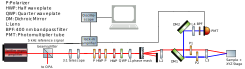
\includegraphics[width=\textwidth]{gfx/ch3/pdf/setup.pdf}
\caption{asdf}
\end{figure}

Finally, the polarized output reflects off of two dichroic mirrors (oriented in such a way as to cancel the differing effect of the Fresnel equations on the reflectivity of S and P polarized light) and is focused through a $400$ \si{nm} bandpass filter onto a \gls{pmt} by a $400$ \si{mm} lens.
The current output of the \gls{pmt} is filtered by a lock-in amplifier (for static \gls{shg}, set to the $5$ \si{kHz} repetition rate of the laser) and read out on an oscilloscope.
The phase mask, incoming polarizer, and outgoing polarizer are mounted on rotating lens tubes which are connected via pulley to a common motor shaft driven by a brushless DC motor.
The motor thus continuously rotates the plane of incidence of the experiment, since the latter is entirely defined by the phase mask and the polarizers.
The rotation angle is tracked as a function of time by an optical rotary encoder, consisting of a laser pointer passed through a chopper wheel (with 100 slots) mounted at the end of the motor shaft and detected via photodiode.
The encoder signal and the lock-in signal are both sent to a homemade oscilloscope (an Arduino Uno microcontroller which separates the lock-in signal into different individual rotations by looking for peaks in the encoder signal), the output of which is sent to a computer for further data processing.

\chapter{Automated Polarization Rotation for Multi-Axis Rotational-Anisotropy Second Harmonic Generation Experiments}\label{ch:polrotators}
\section{Preface}

This chapter is based on a manuscript intended for standalone publication and modified to fit the format of this thesis.
It was coauthored by myself and Karna Morey (as co-first authors), along with Baiqing Lv, Zongqi Shen, and Nuh Gedik.
Karna Morey and I initiated the project, designed and built the polarization rotators, performed the demonstration experiment, and wrote the paper.
Baiqing Lv and Zongqi Shen contributed to the design and helped review the manuscript.
Nuh Gedik supervised the project.

\section{Abstract}

\gls{rashg} is a nonlinear optical technique used to probe the symmetry of condensed matter systems. 
Measuring the dependence of the SHG susceptibility on one or more external parameters, notably strain, field, temperature, or time delay, is an extremely powerful way to probe complex phases of quantum materials. 
Experimentally, extracting maximal information about the SHG susceptibility tensor requires measurements of S and P polarized input and output combinations, which naturally involves the rotation of the polarizers during data collection.  
For multi-axis experiments, this has proved challenging since polarization rotation is typically done manually. 
Automating this process eliminates labor constraints, reduces uncertainty due to low-frequency noise, and expands the type of multi-axis datasets that can be collected; however, it is difficult due to geometrical constraints within the setup.
In this work, we design and implement low-cost, high-fidelity automated polarization rotators for use in multi-axis \gls{rashg}.
These polarization rotators utilize an electrical slip ring to transfer power to the rotating \gls{rashg} optical setup as well as a miniature stepper motor to perform the polarization rotation.
We demonstrate this automated system in time-resolved \gls{rashg} measurements in the non-centrosymmetric semiconductor \ce{GaAs}. 
For the multi-axis measurements described above, this automated system permits data averaging over longer periods, vastly expedites data collection, and expands the setup measurement capability.
This ultimately opens new frontiers in probing quantum materials using multiple tunable external parameters.

\section{\label{km-sec:intro} Introduction}

Probing the structure of crystalline solids is essential to understanding their intrinsic functionalities. 
Traditionally, diffraction techniques based on the scattering of e.g. x-rays are used to determine this structure; however, these techniques predominantly measure the total electron density and are thus insensitive to long-range ordering of the valence electron subsystem.
In contrast, nonlinear scattering techniques at optical frequencies like \gls{rashg} are sensitive rather to the total charge density, and thus offer a complementary view of the electronic, magnetic, and lattice properties of quantum materials \citep{torchinsky_low_2014, fichera_second_2020}.\footnote{In this paper, we discuss \glsfmtshort{rashg}, although the results are fully generalizable to arbitrary harmonics, e.g. third harmonic generation.}


Furthermore, due to the non-invasive nature of \gls{rashg}, it can also be used to investigate changes along one or more measurement axes, such as strain, field, pressure, temperature, or time delay.
The phase diagram of quantum materials is heavily influenced by these independent variables, and thus, changes to the SHG response along such measurement axes are of great interest.
For example, previous studies have used various continuous experimental parameters such as pressure \citep{li_high-pressure_2022}, time delay\citep{shan_gian_2021}, and magnetic field to investigate phase transitions in quantum materials.
Such measurements can illuminate the roles that charge, spin, and thermal degrees of freedom play within quantum materials.

Second harmonic generation gleans microscopic information through the coupling of an order parameter to the second harmonic susceptibility tensor (at least a third-rank tensor with 18 independent components) \citep{boyd}. 
This tensor governs the relationship between the vector properties (i.e. polarization and intensity) of the incident radiation and the generated second harmonic, as shown in \cref{km-eq:intensity}.
The complexity of this tensor means that a significant amount of data is needed to fully resolve the tensor components, posing experimental challenges with data collection.
The importance of resolving the tensor components can be seen by considering Neumann's principle, which states that these tensors must be invariant under symmetry operations of the material's point group, which constrains the tensors' independent and nonzero elements \citep{birss}. 
By measuring the intensity and polarization of the generated second harmonic radiation, \gls{rashg} provides information about these tensor elements and thus the underlying point group.
When performing experiments with more than one measurement axis, the data constraints mentioned above can often be especially burdensome, limiting the type of experiments that can be performed using \gls{rashg}.
Thus, new methods for collecting data efficiently for multi-axis \gls{rashg} experiments are incredibly important.

\begin{figure}
\centering
\phantomsubfloat{\label{km-fig:1a}}
\phantomsubfloat{\label{km-fig:1b}}
\includegraphics[width=\textwidth]{gfx/ch4/km-fig1.pdf}
\caption[A demonstration of \glsfmtshort{rashg} in the test sample \ce{GaAs}]{
\label{km-fig:1}
\begin{enumerate*}[label=\caplabel, ref=\capref]
\item[] A demonstration of \glsfmtshort{rashg} in the test sample \ce{GaAs}.
\qty{800}{nm} light comes in at an oblique angle of incidence, after being passed through a polarizer.
The polarization axis of the light is in the plane of incidence and is denoted in the insets of the figure with a black arrow.
Depending on the angle of the plane of incidence relative to the crystallographic axes, as well as the polarization of the beam relative to that incoming plane of incidence, the second harmonic response to the stimuli should vary from zero points (nodes) to non-zero maxima.
\end{enumerate*}
}
\end{figure}

A more detailed understanding of the information that needs to be collected to fully resolve the second harmonic susceptibility can be seen by considering \cref{km-fig:1}.
\Cref{km-fig:1} shows a schematic of an \gls{rashg} setup, where near-infrared light from the laser source enters at oblique incidence and is scattered off the front of the sample, generating blue light at the second harmonic frequency.
To leading order, the measured second harmonic intensity is given by
\begin{equation}
I(\phi) = \big| E^{\mathrm{out}}_i(\phi) \chi^{(2)eee}_{ijk} E^{\mathrm{in}}_j(\phi) E^{\mathrm{in}}_k(\phi)\big|^2,
    \label{km-eq:intensity}
\end{equation}
where $\phi$ is the azimuthal angle between the crystallographic axes and the plane of incidence, $E^{\mathrm{out}}$ and $E^{\mathrm{in}}$ are the polarization vectors of the outgoing and incoming light, respectively, and $\chi^{(2)eee}$ is the SHG electric-dipole susceptibility tensor.
For certain values of $\phi$, as shown in \cref{km-fig:1a}, the sample is symmetric with respect to the polarization axis of the incoming light; in this case, the second harmonic generation is constrained to be zero, whereas in general arbitrary angles give a non-zero second-harmonic response (see \cref{fig:1}b).
Neumann's principle dictates that \cref{km-eq:intensity} captures the symmetry considerations shown in \cref{km-fig:1}, i.e. the symmetries of the crystal are embedded into its nonlinear susceptibility tensor $\chi^{(2)}$.

These considerations demonstrate the necessity of measuring the full rotational anisotropy of the SHG response, as well as its dependence on the incoming and outgoing polarization directions (which may be P or S-polarized, leading to four independent polarization channels).
The former requires rotating the plane of incidence, which is typically done by rotating the optical setup itself rather than the sample \citep{petersen_nonlinear_2006,torchinsky_low_2014, fichera_second_2020, camn2bi2}. 
The geometric constraints involved in rotating the optical setup make it challenging to use electromechanical components to rotate the polarizers shown in \cref{fig:1} between S and P configurations, since naively it is difficult to transfer power to the rotating frame of reference.
Because of this, switching between different polarization channels is typically done manually, resulting in time and labor constraints that often limit data collection beyond a single polarization combination \citep{shan_gian_2021}.
Such constraints severely restrict the ability to infer tensor elements from the \gls{rashg} data and limit RA-SHG to studies involving often just a single tuning parameter. 

Previous multi-axis \gls{rashg} studies typically either collected exclusively one polarization channel \citep{shan_gian_2021} (for more than one axis) or simply sacrificed the quantity of collected data and therefore inferred statistics. 
However, these approaches can often miss certain features in \gls{rashg} data that would be apparent if more efficient data-taking methods were available.
For example, phase transitions in which the order parameter couples differently to different polarization channels through the second harmonic susceptibility \citep{camn2bi2} are best characterized by taking the full rotational anisotropy data.
The benefit of collecting all four polarization combinations underscores the appeal of automated polarization control of \gls{rashg} setups.

\begin{figure}
\centering
\includegraphics[width=\textwidth]{gfx/ch4/km-fig2.pdf}
\caption[A diagram of the full second harmonic generation setup]{
\label{km-fig:2}
\begin{enumerate*}[label=\caplabel, ref=\capref]
\item[] A diagram of the full second harmonic generation setup developed and described in \citet{fichera_second_2020}.
Boxed in part of the setup shows the area of interest of this work, where the incoming and outgoing polarization channels are set.
\end{enumerate*}
}
\end{figure}

In this work, we design and implement automated polarization rotators for use in multi-axis \gls{rashg} measurements. 
The devices utilize a miniature stepper motor housed in an electrical slip ring to circumvent the geometrical constraints imposed by the rotating plane of incidence.
In section \ref{km-sec:disc}, we discuss the specific application of automated polarization rotation to time-resolved RA-SHG and show that it not only expedites data collection but also reduces the setup's sensitivity to low-frequency noise. 
The advantages afforded by the automated polarization rotators exist not only for time-resolved measurements but for any measurements where an external parameter is being varied and compound rapidly as multiple parameters are varied at the same time.

\section{Design}
\label{sec:des}

A detailed schematic of the \gls{rashg} setup is shown in figure 2.
Telescoped pulses from a \qty{5}{kHz} pulsed regenerative amplifier (Spectra-Physics Spitfire) are attenuated using a half-waveplate set between two polarizers and then elliptically polarized using a half-waveplate and quarter-waveplate in series. 
The light is then focused by a lens onto a rotating phase mask (which separates the beam into different diffraction orders), and a beam block selects the +1 order beam which is then collimated using another lens (L2).
Finally, the beam passes through a dichroic mirror and a polarizer (P1) before being focused by a third lens (L3) onto the sample.
The reflected radiation is passed through an analyzer (P2) and is redirected using a dichroic mirror periscope, which has equal reflectivity for S and P-polarized light and selects exclusively the \qty{400}{nm} reflected radiation.
The two polarizers (P1 and P2) and the phase mask are mounted on a rotating shaft coupled to an optical rotary encoder.
After the dichroic mirrors, the second harmonic radiation is focused by a final lens (L4) onto a \qty{400}{nm} bandpass filter and photomultiplier tube.
The signal from the photomultiplier tube is sent to a lock-in amplifier synced to the \qty{5}{kHz} pulsed laser reference signal and the amplified signal is then correlated with the signal from the optical rotary encoder using a home-built oscilloscope. 

Importantly, the geometrical constraints introduced by the rotating plane of incidence mean that rotating P1 and P2 between S and P configurations electromechanically is challenging, as power must be transmitted from the stationary laboratory frame to electrical components lying in the rotating frame.

To solve this problem, we utilize a hollow-bore electrical slip ring and a miniature stepper motor, shown in an exploded-view diagram in \cref{km-fig:3a}.
A slip ring uses stationary conductive brushes sliding against a rotating through-bore cylinder to transfer power from a stationary reference frame to a rotating one, as shown in \cref{km-fig:3b} \citep{argibay_asymmetric_2010}. 
To accommodate the further requirement that the beams pass through the entire device unimpeded, we employ an \qty{8}{mm} stepper motor that fits in between the two beams.
\Cref{km-fig:3c} and \cref{km-fig:3d} show a front view of the device, with the wire grid polarizer in the P and S positions, respectively, and the polarization direction of the polarizer shown in arrows on the edge of the polarizer.
A full rendering, to scale, of the automated system within the full setup is shown in \cref{km-fig:6}. 

\subsection{Slip Ring}

Slip rings are a standard electromechanical device for transferring power from a stationary assembly to a rotating assembly.
An inner, rotating part of the slip ring can freely rotate relative to an outer, stationary part without compromising signal or power transmission.
This functionality is enabled by low-friction metal brushes that slide against another set of electrical contacts, allowing free rotation while maintaining good electrical conductivity \citep{argibay_asymmetric_2010}, as shown in \cref{km-fig:3b}.
To allow for the uninterrupted passage of the beams through the device, we use a hollow-bore slip ring (Moflon MT3899-S040-VD) whose \qty{38}{mm} inner bore rotates along with the lens tube-pulley assembly shown in \cref{km-fig:6}.
Either set screws located on the front side of the slip ring (as shown in \cref{km-fig:3}) or a 3D-printed cylindrical hollow bore adapter (not shown) can secure the inner bore of the slip ring to the lens tube.

\begin{figure}
\centering
\phantomsubfloat{\label{km-fig:3a}}
\phantomsubfloat{\label{km-fig:3b}}
\phantomsubfloat{\label{km-fig:3c}}
\phantomsubfloat{\label{km-fig:3d}}
\includegraphics[width=\textwidth]{gfx/ch4/km-fig3.pdf}
\caption[Exploded-view diagram of one of the automated polarization rotators]{
\label{km-fig:3}
\begin{enumerate*}[label=\caplabel, ref=\capref]
\item An exploded-view diagram of one of the automated polarization rotators, with the individual components labeled.
Each of these is a manufactured part except for the 3D-printed mount.
\item A schematic of the interior of an electrical slip ring, where low-friction metal brushes allow for electrical conduction across a rotating assembly.
\item A front view of the device, in the P-polarized state, with arrows on the edge of the polarizer indicating the polarization direction.
\item Same as \cref{km-fig:3c}, but in the S-polarized state.
\end{enumerate*}
}
\end{figure}

\subsection{Miniature Stepper Motor}
\label{km-sec:stepper}
The hollow bore slip ring allows for the transfer of power to the rotating shaft.
To rotate the wire grid polarizer between S and P configurations while also allowing both beams to pass through the entire device, we use an \qty{8}{mm} diameter Faulhaber Series AM0820 stepper motor.
The stepper motor's shaft is epoxied to a \qty{1}{inch} square wire-grid polarizer roughly \qty{5}{mm} from the closest horizontal and vertical edges, as shown in \cref{km-fig:3c} and \cref{km-fig:3d}.
The stepper motor is mounted in the center of the SM1L15 lens tube using a custom, 3D printed mount as shown in \cref{km-fig:3a}. 
This mount, along with careful epoxying of the polarizer to the motor shaft, ensures that the incidence angle of the beam is close to normal.
Furthermore, the mount ensures that the stepper motor's shaft is aligned closely to the central rotation axis of the entire assembly, minimizing torques on the motor and polarizer.
This stepper motor can support up to \num{800} total micro-steps per revolution (\ang{0.45} per micro-step) and \qty{0.65}{mNm} of holding torque, and is small enough to fit in between the incoming and outgoing beams. 

The motor can then move the polarizer between the P configuration (\cref{km-fig:3c}) and the S configuration (\cref{km-fig:3d}) without manual intervention or the need to stop the rotation of the entire assembly.
The offset placement of the polarizer on the motor shaft allows only one of the beams (either incoming or outgoing) to pass through the polarizer.
The SM1AB2 and SM1P1 adapter pieces allow for arbitrary rotation relative to the longer lens tube-pulley assembly, allowing the beams to be aligned with the empty spaces in the stepper motor mount.
These adapter pieces also allow for small ($\pm \ang{20}$) rotations of the polarizer about the central axis to account for factory defects which may cause the polarization axis to be misaligned with the straight edges of the polarizer.

\begin{figure}
\centering
\includegraphics[width=\textwidth]{gfx/ch4/km-fig4.pdf}
\caption[A 3-dimensional rendering of the automated polarization rotators]{
\label{km-fig:6}
\begin{enumerate*}[label=\caplabel, ref=\capref]
\item[] A 3-dimensional rendering of the boxed-in part of the setup in \cref{km-fig:2}, with fully automated polarization rotators.
\end{enumerate*}
}
\end{figure}

Another copy of the same system shown in \cref{km-fig:3} is mounted on the other side of the lens tube-pulley assembly and controls the polarization of the reflected beam, as shown in \cref{km-fig:6}. 
The back sides of both devices, shown in \cref{km-fig:6}, are attached to the rotating lens tube-pulley-motor-shaft assembly shown in \cref{km-fig:6} via threads on the long central lens tube. 
A hole drilled in the top and bottom of the SM1L15 piece in each device shown in figure \cref{km-fig:3a} allows feedthrough wires to connect the four leads of the stepper motor to the four rotating inner-bore slip ring leads.
The four leads on the stationary side of each slip ring directly connect to a Geckodrive G250X digital step driver for each device, controlled by a single Arduino Nano Every.
This control circuit allows for the integration of the stepper motors with existing instrumentation software.

Whenever the stepper motors lose power, the polarizers need to be re-aligned due to the loss of their holding torque.
The alignment is performed by using a reference polarizer with a known polarization axis.
First, the plane of incidence of the entire assembly is positioned to the known polarization plane of the reference polarizer, then the polarizers themselves can be oriented by placing the beam through the reference polarizer and rotating the stepper motor until beam extinction (yielding an S-polarized alignment).  
The polarizers can then freely rotate between this S-polarized position and the orthogonal P-polarized position.

\section{Validation and Discussion}
\label{km-sec:disc}

\begin{figure}
\centering
\includegraphics[width=\textwidth]{gfx/ch4/km-fig5.pdf}
\caption[Demonstration of the automatic polarization rotators]{
\label{km-fig:4}
\begin{enumerate*}[label=\caplabel, ref=\capref]
\item[] A polar plot of the change in SHG intensity (from the pre-pump state) as a function of time since zero-delay for the test sample GaAs.
This is a demonstration of using the automated polarization rotators to take \gls{trshg} data.
\qty{55} different pump-probe delays (only four time delays are plotted) were taken in this dataset, meaning that \qty{220} polarization rotations were performed using the automated polarizers.
\end{enumerate*}
}
\end{figure}

To test these automated polarization rotators, we performed time-resolved RA-SHG on the non-centrosymmetric semiconductor \ce{GaAs} \citep{ducuing_observation_1963, torchinsky_low_2014}. 
A pump line was added to the setup shown in \cref{km-fig:2} by mounting a \ang{45} mirror onto L3 so that the pump beam may be reflected directly onto the sample. 
The pump pulse is produced by an optical parametric amplifier (Spectra-Physics Topas) tuned to a wavelength of \qty{1.3}{\mu m}.
The pump line includes a delay stage, which controls the relative time delay between the pump and the probe pulses, and a chopper wheel, which reduces the effective repetition rate of the pump pulses to \qty{2.5}{kHz}. 
With the pump repetition rate of \qty{2.5}{kHz} and the probe repetition rate of \qty{5}{kHz}, locking in at a frequency of \qty{2.5}{kHz} produces a signal proportional to the change in the \gls{shg} intensity relative to equilibrium.
For time-resolved measurements on \ce{GaAs}, shown in \cref{km-fig:4}, \qty{55} different pump-probe delays were taken, resulting in \qty{220} different automatic rotations of the polarizers.
The data in \cref{km-fig:4} shows the change in the \gls{shg} intensity relative to equilibrium as a function of the pump-probe delay, for each of the polarization channels. 
The use of the polarization rotators in this validation measurement demonstrates their functionality and broad utility for multi-axis \gls{rashg} measurements.

This system was also used to expedite data collection in recent studies of time-resolved, temperature-dependent \gls{rashg} \citep{camn2bi2}.
This particular type of \gls{rashg} measurement demonstrates the general advantages of automated polarization control in multi-axis \gls{rashg} measurements.
To see this, note that if the rotation of the polarizers is performed manually, the best data-taking strategy involves taking the time dependence of one polarization channel in full before moving to the next. 
However, in the presence of low-frequency noise (due to e.g. fluctuations in the laser intensity), this is problematic as the different polarization channels will not be taken under equivalent conditions. 
In the automated case, in contrast, all polarization channels can be taken at each time delay. 
This greatly decreases the experiment's susceptibility to low-frequency noise and expedites data taking by allowing for overnight and multi-day scans.

Automated polarization rotation thus vastly improves RA-SHG data collection, eliminating the need for manual polarization rotation, especially in cases of multiple experimental axes. 
The roughly \qty{1,000}{\$} total cost of both devices (not including polarizers) makes them relatively inexpensive, and the design is easily implementable in existing \gls{rashg} setups.
Multi-axis measurements are becoming increasingly important to resolve complicated phase diagrams and competing orders, and thus future measurements will increasingly rely on automated systems such as the one presented in this work.

\chapter{Second harmonic generation as a probe of broken mirror symmetry in 1\textit{T}-\ce{TaS2}}\label{ch:tastwo}
\chapter{Light-induced reorientation transition in the antiferromagnetic semiconductor \ce{CaMn2Bi2}}\label{ch:cmb}
\chapter{Amplitude-mode electromagnon in the XXZ chain \ce{CuBr2}}\label{ch:cubr2}
\chapter{Concluding remarks}\label{ch:conclusion}

\backmatter*
\bibliography{fichera-bfichera-phd-physics-2024-source}

\end{document}
